% Created 2017-03-01 Wed 20:38
\documentclass[10pt]{article}
\usepackage[utf8]{inputenc}
\usepackage[T1]{fontenc}
\usepackage{fixltx2e}
\usepackage{graphicx}
\usepackage{longtable}
\usepackage{float}
\usepackage{wrapfig}
\usepackage{rotating}
\usepackage[normalem]{ulem}
\usepackage{amsmath}
\usepackage{textcomp}
\usepackage{marvosym}
\usepackage{wasysym}
\usepackage{amssymb}
\tolerance=1000
\usepackage{natbib}
\usepackage[linktocpage,pdfstartview=FitH,colorlinks,
linkcolor=blue,anchorcolor=blue,
citecolor=blue,filecolor=blue,menucolor=blue,urlcolor=blue]{hyperref}
\usepackage[margin=2cm]{geometry}
\pagenumbering{gobble}
\usepackage{wrapfig}
\usepackage{multicol}
\setlength\columnsep{20pt}
\author{Alejandro Rodríguez Salamanca - r0650814 - Erasmus}
\date{}
\title{Character recognition with Hopfield networks}
\begin{document}

\maketitle

\begin{multicols}{2}

  \section*{Data preparation}
  Before starting to solve the tasks, the dataset to use must be
  constructed. For this exercise, we are asked to pre-pend the
  lowercase characters of our first and last name to the set of
  capital characters given in \texttt{prprob}. As my name is
  Alejandro Rodriguez, the characters I have to pre-pend are:
  \texttt{a, l, e, j, n, d, r, o, i, g, u, z}. Once this is done,
  it's time to solve the three proposed problems.

  \section*{Task 1: Retrieve the first 5 characters.}
  The first 5 characters of the alphabet are \texttt{a, l, e, j}
  and \texttt{n}, this is, the first five characters that appear in
  my first name and last name. After loading this characters, the
  pixels whose value is 0 must be changed by -1. This has to be done
  because Hopfield nets normally have units that take on values of
  1 or -1 as convention.

  % Image of the characters
  \begin{center}
    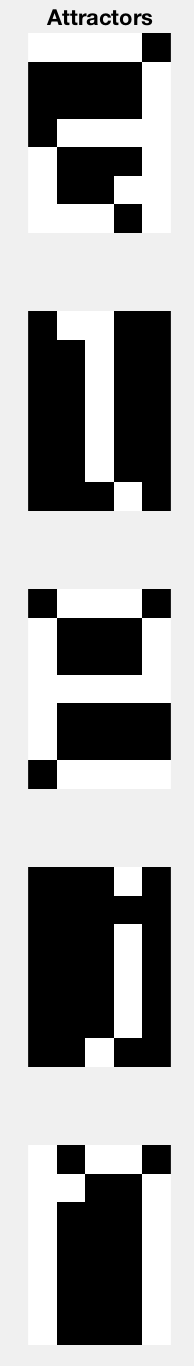
\includegraphics[height=\linewidth]{img/chars1}
  \end{center}

  With this five characters as attractor states, a Hopfield neural
  network is created. Then, three random pixels of each character
  are inverted (from 1 to -1 and viceversa). The objective of this
  inversion is to check if the network is able to reconstruct the
  distorsioned characters.

  Executing the neural network with the noisy characters as input
  shows the following results:

  \begin{itemize}
  \item With a small number of steps: it can be seen that the
    characters are being attracted by the attractor states, but they still
    contain some noise.
    % Image with 2 steps
    \begin{center}
      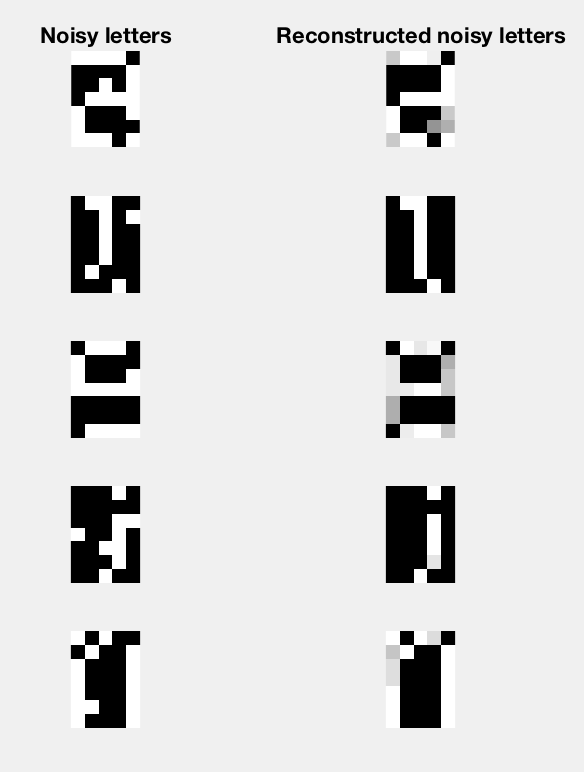
\includegraphics[height=\linewidth]{img/recons1}
    \end{center}
  \item When the number of steps is increased: with just 5 steps, the
    characters are perfectly reconstructed.
    % Image with 5 steps
    \begin{center}
      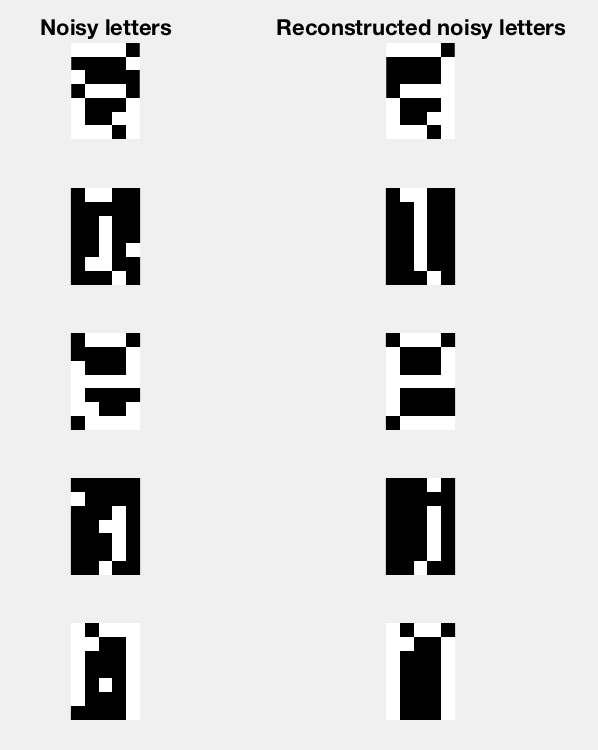
\includegraphics[height=\linewidth]{img/recons2}
    \end{center}
  \end{itemize}

  Sporious patters are local energy minima that are created during
  training, in addition to the intended target patterns. They are
  activity patterns that have not been explicitly embedded in the
  synaptic matrix, but are nonetheless stable. They are in other
  words "unwanted" attractor states that, by virtue of a finite
  overlap with the "wanted" attractor states, come about as a
  local minimum in the energy function. In this case, the existence
  of sporious patters is not noticeable.

  \section*{Task 2: Critical loading capacity}
  A Hopfield neural network exceed the loading capacity when the number of
  learned patterns over number of units $p/N$ is lower than the critical
  capacity $\alpha \approx 0.138$.
  First, a number $P = 20$ characters is selected, and the error in the
  reconstruction is calculated as a function of the number of steps used
  to reconstruct the character.

  \begin{center}
    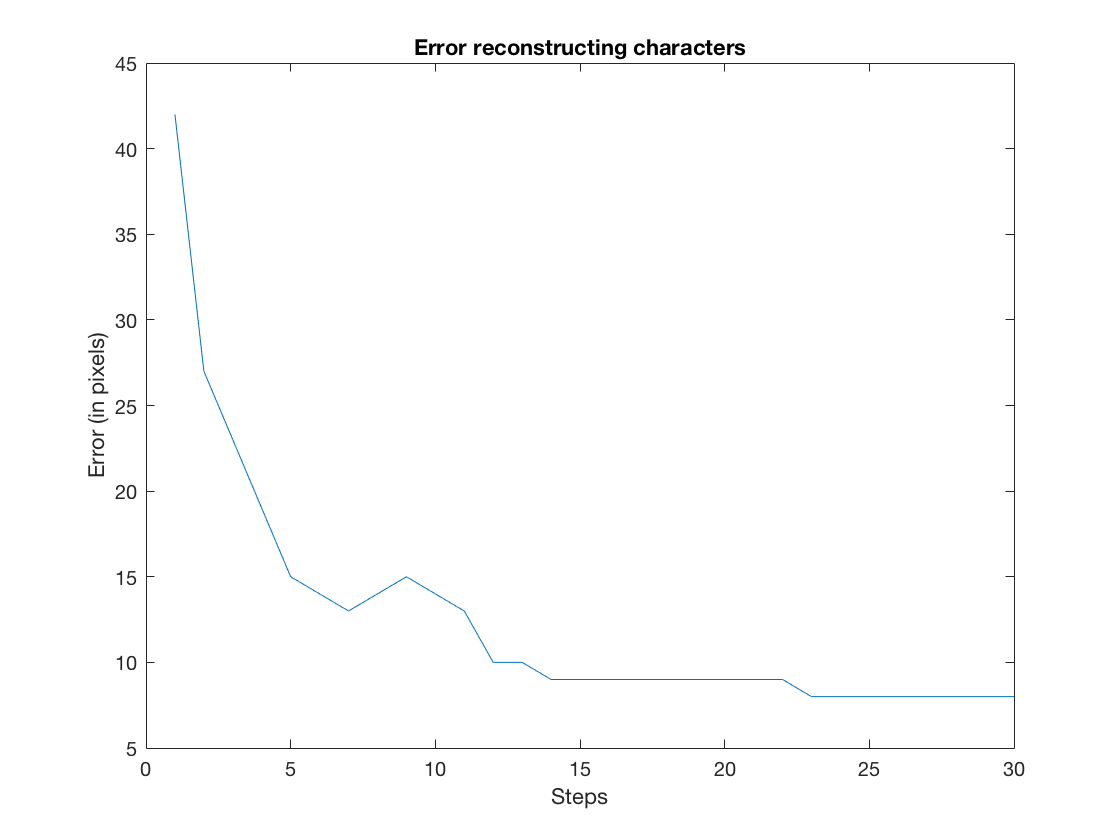
\includegraphics[height=0.8\linewidth]{img/plot_error1}
  \end{center}

  The purpose of this plot is to see how the approximation becomes more
  accurate when the number of steps is increased. Now, let's see what
  happens when the number of characters varies while keeping the number
  of steps fixed at 15.

  \begin{center}
    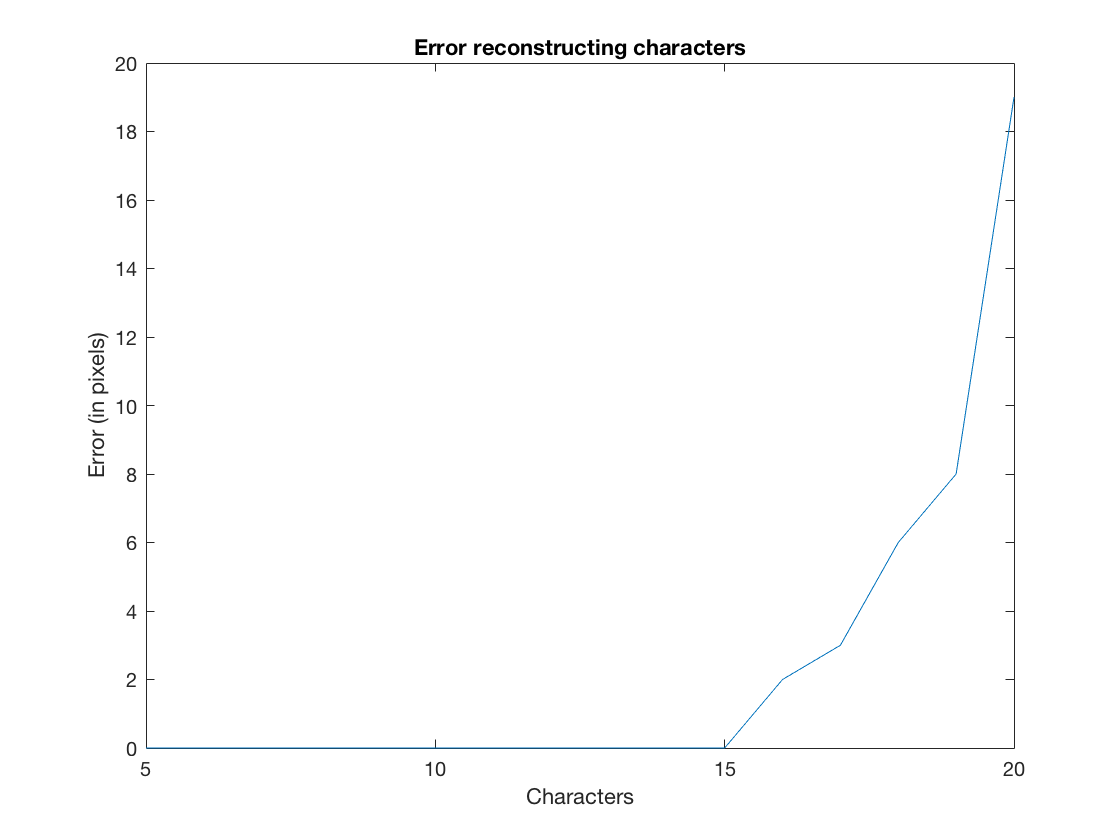
\includegraphics[height=0.8\linewidth]{img/plot_error2}
  \end{center}

  The critical capacity of a Hopfield network, as stated before, is $p/N$,
  where $p$ is the set of patterns to be memorized and $N$ the number
  of neurons. The number of neurons is determined by the number of pixels
  in each image. The dimension of each image is $7 \times 5$, which means that
  the number of neurons of the network is 35.

  Now, the critical capacity can be expressed as $p/35$. 
  
  
  \section*{Task 3: Retrieve 25 characters}
  
  %https://en.wikipedia.org/wiki/Hopfield_network
  %https://cogsci.stackexchange.com/questions/903/spurious-attractors-in-hopfield-networks
  %https://www.quora.com/What-are-spurious-states-in-Hopfield-networks

\end{multicols}

  \section*{Appendix}

\end{document}
